\subsection{Somme connexe}

\begin{definition}[Somme connexe]
Soient $X$ et $Y$ deux $n$-variétés lisses. Soient $B_X \subset X$ et $B_Y \subset Y$ des boules ouvertes plongées de façon compatible avec l'orientation. On définit la \textbf{somme connexe} de $X$ et $Y$ par
\[
X \# Y \;=\;  (X \setminus B_X) \cup_{\varphi} (Y \setminus B_Y) \;=\; \bigl(X \setminus B_X\bigr) \sqcup \bigl(Y \setminus B_Y\bigr) \big/ \sim
\]
où $\sim$ identifie chaque point $x \in \partial \overline{B_X}$ avec $\varphi(x) \in \partial \overline{B_Y}$, et $\varphi : \partial \overline{B_X} \xrightarrow{\;\sim\;} \partial \overline{B_Y}$ est un difféomorphisme \emph{renversant l'orientation} (de sorte que les orientations de $X\setminus B_X$ et $Y \setminus B_Y$ induisent une orientation cohérente sur $X\#Y$).
\end{definition}

\begin{figure}[h]
  \centering
  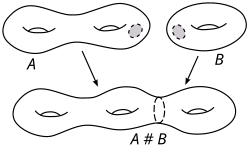
\includegraphics[width=0.7\textwidth]{connected_sum.png}
  \caption{Somme connexe de deux variétés}
  \label{fig:somme-connexe}
\end{figure}

\subsubsection*{Homologie de la somme connexe}

\begin{proposition}
Soient $X$ et $Y$ deux $n$-variétés lisses. On a un isomorphisme
\[
H_2(X \# Y) \cong H_2(X) \oplus H_2(Y).
\]
\end{proposition}

\begin{proof}
Soient $B_X \subset X$ et $B_Y \subset Y$ des boules ouvertes. Posons
\[
X' = X \setminus B_X, \qquad Y' = Y \setminus B_Y.
\]
Alors $X \# Y = X' \cup_{\varphi} Y'$ où $\varphi : \partial X' \to \partial Y'$ est un difféomorphisme renversant l'orientation, avec $\partial X' \cong \partial Y' \cong S^3$.

Appliquons la suite de Mayer-Vietoris pour le recollement le long de $S^3$ :
\[
\cdots \to H_k(S^3) \to H_k(X') \oplus H_k(Y') \to H_k(X \# Y) \to H_{k-1}(S^3) \to \cdots
\]

Pour $k = 2$, on a $H_2(S^3) = 0$ et $H_1(S^3) = 0$. La suite se réduit à la suite exacte courte :
\[
0 \to H_2(X') \oplus H_2(Y') \to H_2(X \# Y) \to 0.
\]
Ainsi $H_2(X \# Y) \cong H_2(X') \oplus H_2(Y')$.

En dimension $4$, le retrait d'une boule ne modifie pas $H_2$ : $H_2(X') \cong H_2(X)$ et $H_2(Y') \cong H_2(Y)$. En effet :

Montrons que $H_2(X') \cong H_2(X)$. Considérons la paire $(X, X')$. Par excision,
\[
H_2(X, X') \cong H_2(\overline{B_X}, \partial B_X).
\]
La suite exacte de la paire $(\overline{B_X}, \partial B_X)$ donne, puisque $\partial B_X \cong S^3$ et $H_2(S^3)=0$,
\[
0 \to H_2(\overline{B_X}) \to H_2(\overline{B_X}, \partial B_X) \to H_1(S^3)=0,
\]
donc $H_2(\overline{B_X}, \partial B_X) \cong H_2(\overline{B_X}) = 0$ car $\overline{B_X}$ est contractile. Ainsi $H_2(X, X') = 0$.

La suite exacte longue de la paire $(X, X')$ donne alors :
\[
H_2(X') \to H_2(X) \to 0,
\]
et la flèche $H_2(X') \to H_2(X)$ est surjective. De plus, la suite exacte en degré $3$ donne :
\[
H_3(X) \to H_3(X, X') \to H_2(X') \to H_2(X) \to 0.
\]
Or $H_3(X, X') \cong H_3(\overline{B_X}, \partial B_X) \cong H_2(\partial B_X) \cong H_2(S^3)=0$, donc $H_2(X') \to H_2(X)$ est aussi injective. Ainsi $H_2(X') \cong H_2(X)$.

\end{proof}

%==============================================================================